\documentclass{article}%
\usepackage[T1]{fontenc}%
\usepackage[utf8]{inputenc}%
\usepackage{lmodern}%
\usepackage{textcomp}%
\usepackage{lastpage}%
\usepackage[head=40pt,margin=0.5in,bottom=0.6in]{geometry}%
\usepackage{graphicx}%
%
\title{\textbf{HRW advirtió de un empeoramiento de los derechos humanos en Latinoamérica}}%
\author{EFE}%
\date{07/12/2018}%
%
\begin{document}%
\normalsize%
\maketitle%
\textbf{URL: }%
http://www.el{-}nacional.com/noticias/latinoamerica/hrw{-}advirtio{-}empeoramiento{-}los{-}derechos{-}humanos{-}latinoamerica\_262500\newline%
%
\textbf{Periodico: }%
EN, %
ID: %
262500, %
Seccion: %
Latinoamérica\newline%
%
\textbf{Palabras Claves: }%
NO\_TIENE\newline%
%
\textbf{Derecho: }%
5, %
Otros Derechos: %
1.10, %
Sub Derechos: %
1.10.1.1\newline%
%
\textbf{EP: }%
NO\newline%
\newline%
%
\textbf{\textit{José Miguel Vivanco, director para las Américas de la ONG, advirtió~que esto constituye "un problema muy serio" en países como México, Brasil o Venezuela}}%
\newline%
\newline%
%
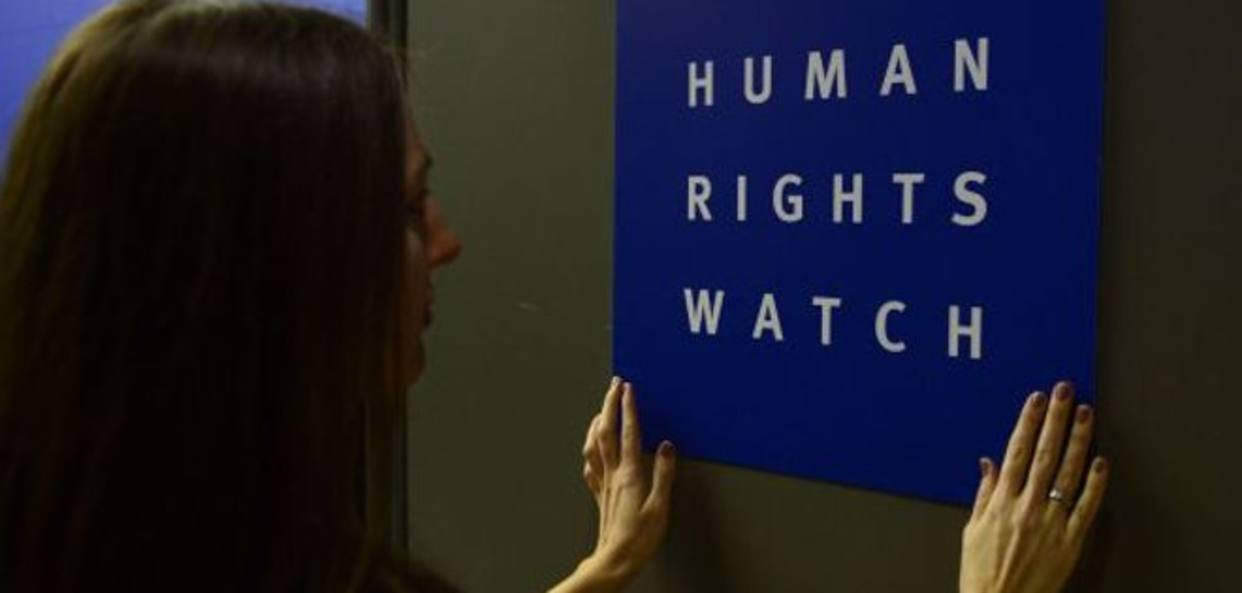
\includegraphics[width=300px]{189.jpg}%
\newline%
%
El director para las Américas de la ONG Human Right Watch (HRW), José Miguel Vivanco, dibuja un oscuro presente para los~derechos humanos~en~Latinoamérica~y~adviertió~sobre su "empeoramiento" en el futuro cercano.%
\newline%
%
"Se viene un periodo complejo, entramos en una etapa compleja, difícil, aún más difícil que la que hemos enfrentado desde el punto de vista de los~derechos~humanos", asegura Vivanco en una entrevista con Efe tras concluir en Nueva York unas jornadas de reflexión de su ONG.%
\newline%
%
En su conversación, Vivanco desgrana los que a su juicio son los problemas más graves que afrontan muchos de los países de la región, aunque dejó~claro que existen realidades "muy distintas" en~Latinoamérica.%
\newline%
%
"Entre las cuestiones que son preocupantes, lo primero que me parece necesario destacar es el tema de la inseguridad, el crimen organizado y la criminalidad", asegura el responsable de HRW, que hace hincapié en lo duro de su trabajo, "donde normalmente, lo usual es perder, no ganar".%
\newline%
%
Para Vivanco, muchas veces, la respuesta a esta inseguridad que, "en distintos grados", preocupa a toda la zona, "es la mano dura, y con argumentos demagogos de que el incremento de penas, la militarización de la policía o el descenso de la edad penal" contribuyen a su mejora.%
\newline%
%
Desde HRW consideran que estas medidas son "una fuente de abusos casi inagotable", con un aumento de "la brutalidad y prácticas como la tortura, ejecuciones y cárceles repletas de procesados sin condena".%
\newline%
%
El responsable para la Américas de HRW~advirtió~de que esto constituye "un problema muy serio" en países como México, Brasil o en Venezuela, país este último "con las tasas de homicidios y de delitos violentos más alta", así como en Centro América, por el problema de la "violencia brutal" de las maras en Honduras, El Salvador o Guatemala.%
\newline%
%
"Frente a esto, muy pocos países han encontrado una respuesta profesional y que genere confianza sin que signifique más violaciones", subraya.%
\newline%
%
Vivanco, para quien "lo que empuja (a un trabajador humanitario) es un elemental principio de solidaridad con los más vulnerables", va más allá y cree que otro grave problema en la zona es el "surgimiento de gobiernos civiles populistas" como el de Nicolás Maduro en Venezuela y el de Daniel Ortega en Nicaragua.%
\newline%
%
"Venezuela y Ortega ven en Cuba un modelo y caminan abiertamente en esa dirección. La clave es impedir que se consoliden dictaduras propias de los 70. Aún no lo han logrado, pero están muy cerca de hacerlo", dice, antes de acentuar que en solo tres meses de represión en Nicaragua en 2018 murieron más del doble de personas que en Venezuela en los últimos años.%
\newline%
%
El directivo chileno de HRW sostiene que la opinión pública debe entender que en la lucha por la defensa de los~derechos~humanos~no puede haber un "doble rasero", insistiendo en que hay que perseguir las violaciones tanto en países con gobiernos de derechas como de izquierdas, populistas o con legitimación popular.%
\newline%
%
"Todos tienen que estar sujetos a las mismas reglas, si uno hace la vista gorda hacia algunas violaciones, ese es probablemente el principal cáncer contra el avance de los~derechos~humanos~a nivel global", sentencia.%
\newline%
%
Además de los "fenómenos extremos" de Venezuela o Nicaragua, Vivanco~advierte~contra el surgimiento de "líderes populistas fundamentalistas" en "los países más grandes", como el presidente de México, Andrés Manuel López Obrador, y el brasileño Jair Bolsonaro, a quienes acusa de no tener "conciencia de respetar las reglas del juego democrático".%
\newline%
%
"Están convencidos de que su sola presencia y el ejercicio del poder les permitirá abordar los graves problemas de esos países", agrega Vivanco: "El ciudadano está en la indefensión total y expuesto al ejercicio arbitrario del poder".%
\newline%
%
Otras cuestiones denunciadas por HRW en la región es la violencia de género o la persecución de periodistas y minorías, como los indígenas o la comunidad LGTBI.%
\newline%
%
Desde "el punto de vista jurídico y de las políticas públicas, cada vez se progresa más en el respeto y los~derechos~de la comunidad LGTBI", pero apunta que "esto aún va acompañado de incidentes de violencia y discriminación muy serios y muy graves".%
\newline%
%
Asimismo, agrega: "Los indígenas no han logrado, lamentablemente, los avances de la comunicad LGTBI y siguen siendo en muchos de nuestros países los más pobres".%
\newline%
%
Más allá de estas malas prácticas y violaciones, Vivanco pone en valor al actual presiente peruano, Martín Vizcarra, por "restablecer los principios de la lucha contra la corrupción", o al presidente ecuatoriano, Lenin Moreno, por sus esfuerzos "notables" y "por mejorar las condiciones de los~derechos~humanos~y para restablecer los~derechos~democráticos que fueron pisoteados por (su antecesor) Rafael Correa".%
\newline%
%
Finalmente, Vivanco también resalta el caso de Costa Rica, que para el directivo de HRW "sigue siendo un importante aliado en la promoción de los~derechos~humanos"%
\newline%
%
\end{document}